\begin{blocksection}
\question
Consider the following 16-bit representation for floating point numbers:
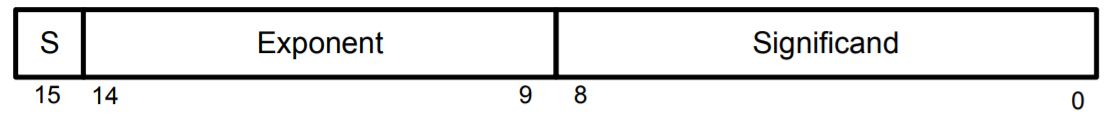
\includegraphics[width=\textwidth]{images/midterm2/floatingpoint.png}

Bits per field:
\begin{itemize}
    \item Sign: 1
    \item Exponent: 6
    \item Significand: 9
\end{itemize}
Everything else follows the IEEE standard 754 for floating point, except in 16 bits.
The bias is \textbf{-31}.

\question
Convert -15.125 into floating point. Write your answer in hexadecimal.
\begin{solution}
\lstinline$0xB5B8$
\end{solution}


\question
What is the value of the largest odd number that can be represented by the above floating point representation?
\begin{solution}
2^10 - 1
\end{solution}


\question
How many positive, real numbers can be represented?
\begin{solution}
2^15 - 2^9 - 1
\end{solution}

\end{blocksection}